\section{Conclusion}
The wireframe renderer works to a degree that allows models to be rendered as wireframes (if they are hardcoded). Because of the problem with screen point calculations (and no clipping), rendering an entire scene is problematic with the current implementation. Navigating a scene is also rather cumbersome due to the poor camera controls. A mouse implementation would offer a large improvement.

\begin{figure}[h!]
  \centering
    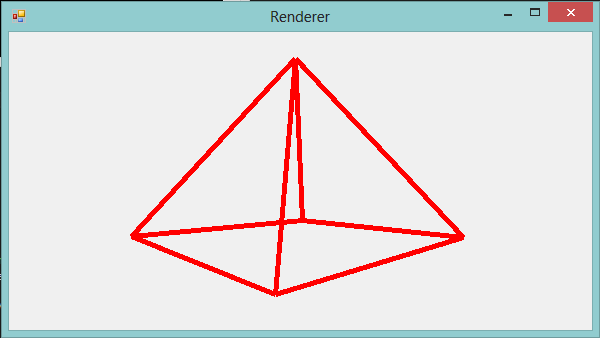
\includegraphics[width=0.35\textwidth]{Screenshots/StartingPosition}
  \caption{The starting position of the renderer.}
\end{figure}

\subsection{Performance}
The hardcoded pyramid contains 5 vertices and 4 triangles, which limits the amount of necessary calculations per call to the \textit{Renderer\_Paint} method. This limits the impact that can be felt from the lack of culling / clipping (even if the camera is away from the view object). To properly test the impact, there would need to be more than one object and/or more complex objects.